\task{На салфетке}

\begin{itemize}
\itA Смотреть рисунок:

\begin{multicols}{2}

\begin{center}
	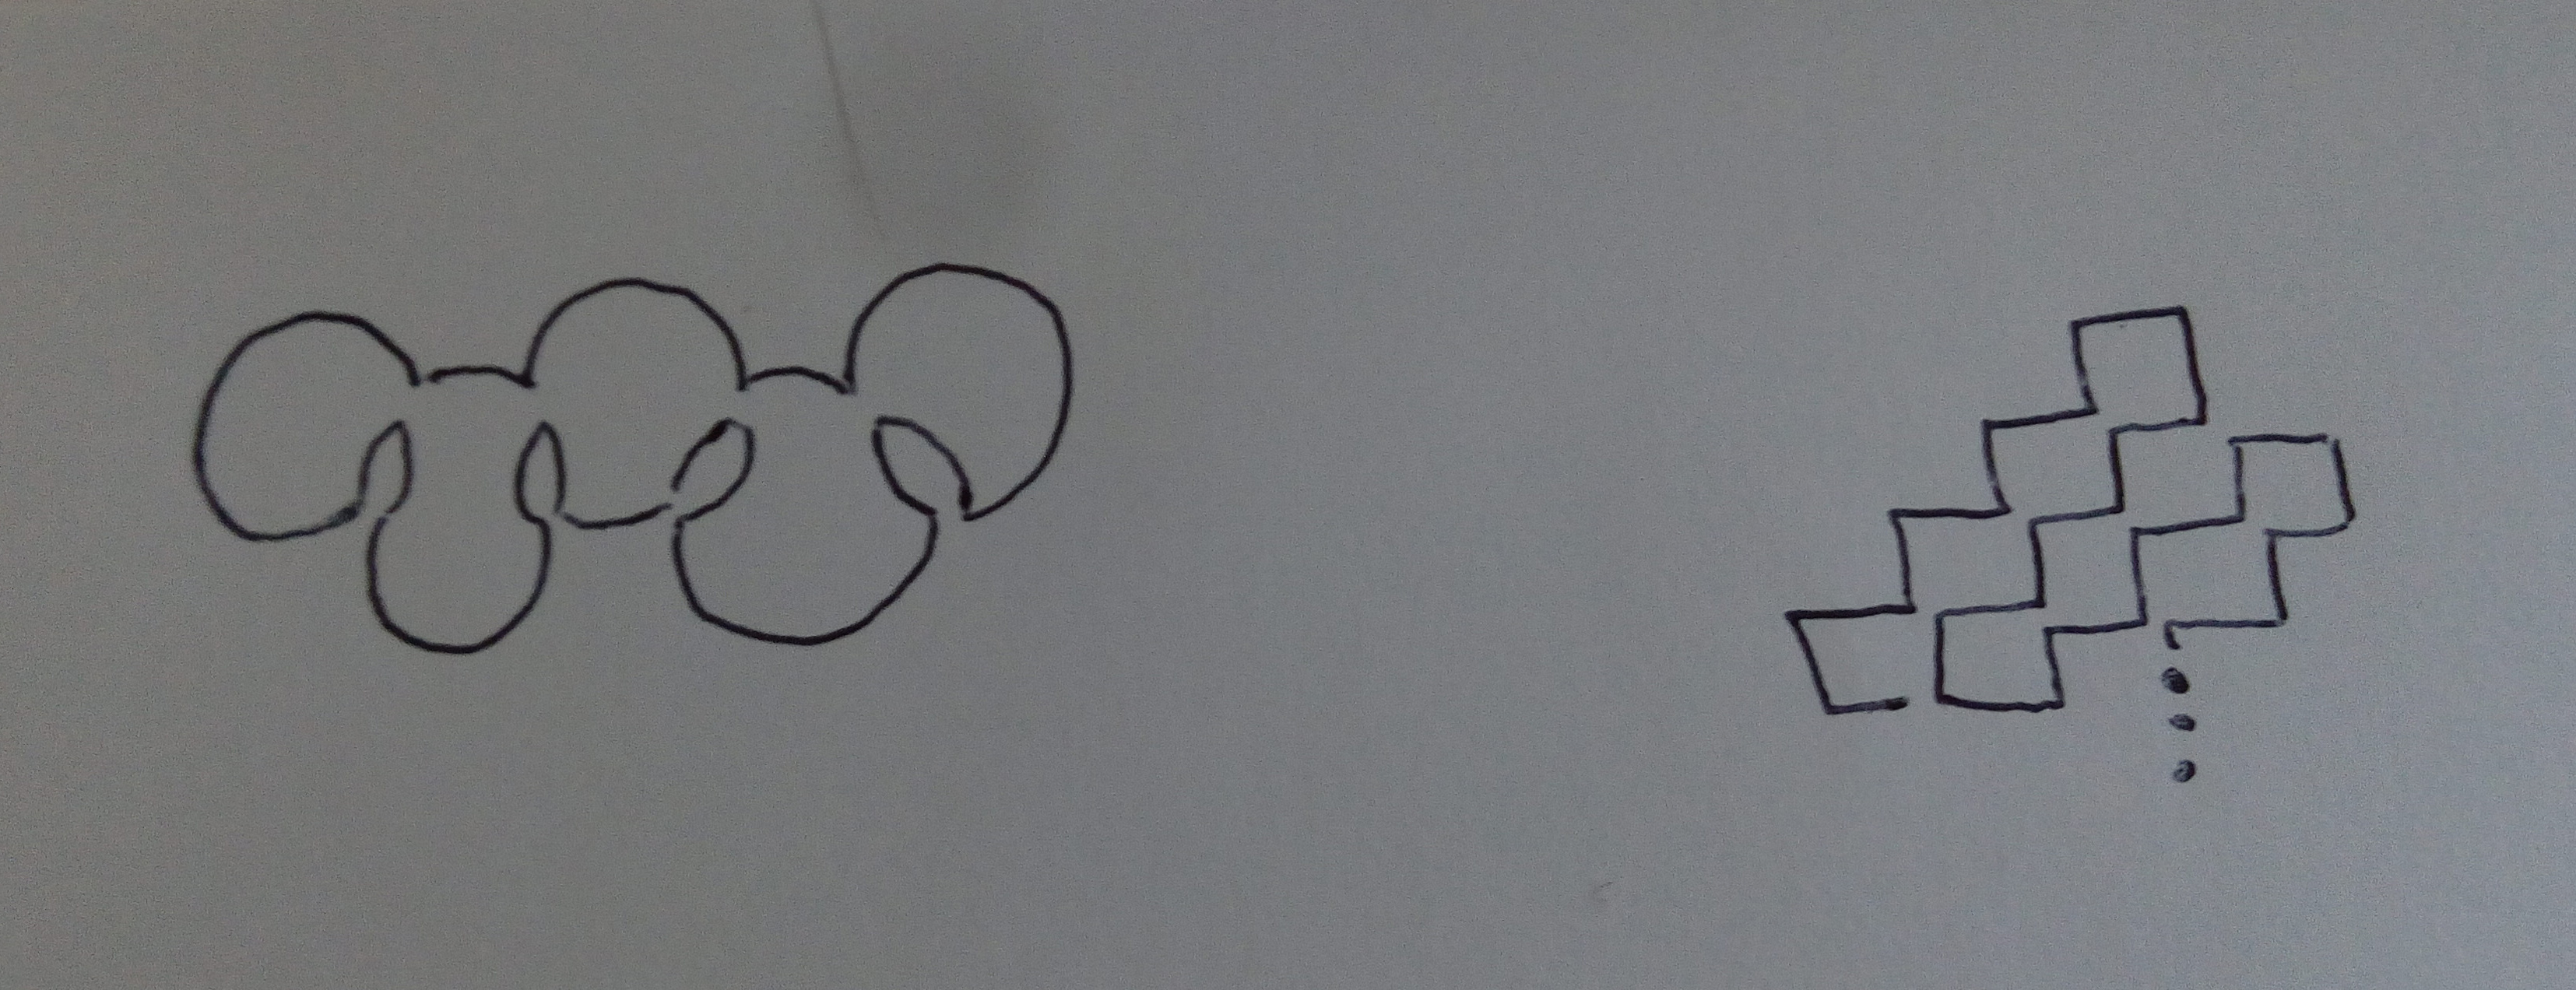
\includegraphics[width=4.4cm]{figures/2018-serpinsky-a}
\end{center}

\columnbreak

\begin{center} \tikz{
\foreach \t in {0,...,3} {
	\draw[thick] (0.6 * \t cm, -0.6 * \t cm) -- ++(0.55,0) -- ++(0,0.5)
		-- ++(0.5,0) -- ++(0,0.5)
		-- ++(0.5,0) -- ++(0,0.5)
		-- ++(0.55,0) -- ++(0,-0.55)
		-- ++(-0.5,0) -- ++(0,-0.5)
		-- ++(-0.5,0) -- ++(0,-0.5)
		-- ++(-0.5,0) -- ++(0,-0.55);};
\draw[thick] (0,0) -- (-0.03,0) -- (-0.03,-0.03);
\draw[thick] (2.33,-2.43) -- (2.4,-2.43) -- (2.4,-2.4);
\foreach \t in {0,...,3} {
	\draw[thick] (-0.03cm + 0.6*\t cm,-0.03cm - 0.6*\t cm)
		-- ++(0,-0.6) -- ++(0.6,0);};
} \end{center}

\end{multicols}


\itB Обозначим количество узлов у треугольника Серпинского степени $n$ через $T(n)$.

У треугольника степени 1 — три узла, $T(1)=3$. Треугольник степени $k+1$ получается из  трёх треугольников степени $k$ поставновкой их друг на друга — при этом три пары узлов (посередине сторон нового треугольника) склеиваются в просто три узла. Таким образом,

\begin{align*}
	& T(k) = 3T(k-1) - 3 =\\
	=\, & 3(3T(k-2)-3)-3 = \ldots = \\
	=\, & 3^{k-1}\cdot T(1) - 3^{k-1} - 3^{k-2} - \ldots - 3 = \\
	=\, & 3^k - 3^{k-1} - 3^{k-2} - \ldots - 3 = \\
	=\, & 3^k - \frac{3^k-1}{3-1} = \frac{3^k+1}{2}. \\
\end{align*}

\vspace{-0.4cm}
Посчитать количество отрезков в наклонном квадрате и того проще: они образуют $2n$ «лесенок», в каждой из которых по $2n$ отрезков. Поэтому ответом будет число $4n^2$.

\itC Научиться рисовать треугольник Серпинского, не отрывая пера от бумаги, можно последовательно: сначала первую степень, потом вторую, потом третью...

Будем делать так: сначала будем, начиная с нижней стороны треугольника, рисовать все его «внутренности», а потом «замкнём» \linebreak получающуюся картинку двумя верхними сторонами. При этом \linebreak «внутренности» треугольника степени $n+1$ — это трижды «внутренности» треугольника степени $n$.

Таким образом получится изображение треугольника степени 4:

\begin{center} \tikz{
	\draw [thick,rounded corners=4,rotate=180]
		[l-system={Sierpinski triangle, axiom=F-X-X, order=3, step=0.5cm, angle=120}]
		lindenmayer system; 
} \end{center}

а также любой другой степени, по аналогии.
\end{itemize}